\chapter{Изучение приборов дозиметрического контроля} \label{chap2}
\section{Дозиметр ДРГ-01Т1} \label{sect2_1}
\subsection{Назначение} \label{subsect2_1_1}
    Дозиметр ДРГ-01Т1 -- цифровой широкодиапазонный носимый дозиметр мощности 
    экспозиционной дозы фотонного излучения (далее -- дозиметр). Предназначен 
    для измерения мощности экспозиционной дозы на рабочих местах, в смежных 
    помещениях и на территории предприятий, использующих радиоактивные 
    вещества и другие источники ионизирующих излучений, в санитарно-защитной 
    зоне и зоне наблюдения. Кроме того, дозиметр может быть использован для 
    контроля эффективности биологической защиты, радиационных упаковок и 
    радиоактивных отходов, а также измерения мощности экспозиционной дозы в 
    период возникновения, протекания и ликвидации последствий аварийных 
    ситуаций.

    \begin{figure}[ht]
		\centering
		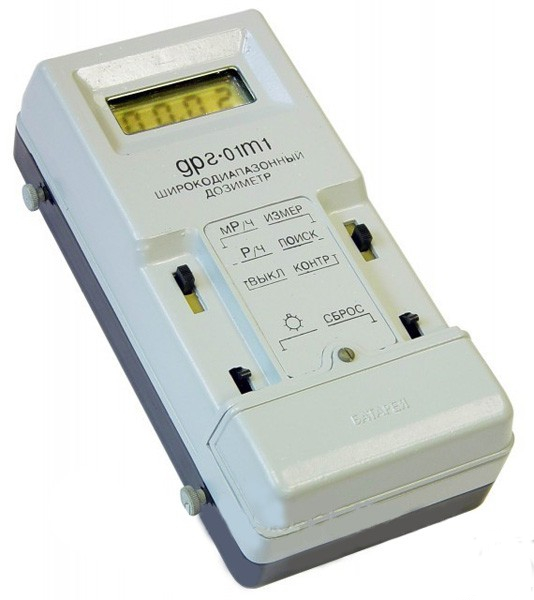
\includegraphics[width=0.3\textwidth]{DRG-01T1.jpg}
		\caption{Внешний вид ДРГ-01Т1}
	\end{figure}

    Дозиметр применяется для оперативного группового контроля мощности 
    экспозиционной дозы работниками служб радиационной безопасности, 
    дефектоскопических лабораторий, санитарно-эпидемиологических станций и
    т.д.

\subsection{Принцип работы} \label{subsect2_1_3}
    В газоразрядных счётчиках под воздействием гамма-квантов генерируются 
    электрические импульсы тока, поступающие на формирователь входного потока 
    импульсов, входной каскад которого преобразует импульсы тока в импульсы 
    напряжения с амплитудой, необходимой для регистрации дальнейшей счётной 
    схемой. С выхода делителя частоты формирователя импульсного потока импульсы 
    поступают на четырёхразрядный счётчик. Накопленная информация за время 
    измерения на счётчике поступает на индикатор через деформацию счётчика 
    в семисегментный позиционный код индикатора.

    Время измерения определяется частотой регулируемого генератора и 
    коэффициентом деления числа импульсов формирователем временного интервала. 
    Изменением времени измерения производится масштабирование входной 
    информации с детекторов в абсолютную величину выходного параметра 
    (мР/ч, Р/ч).

\clearpage

\section{Дозиметр-радиометр ДКС-96} \label{sect2_2}
\subsection{Назначение} \label{subsect2_2_1}
    Дозиметр-радиометр ДКС-06 ТЕ1.415313.003 (далее -- дозиметр-радиометр) 
    изготавливается в соответствии с требованиями ТУ 4362-020-31867313-2008. 

    \begin{figure}[ht]
		\centering
		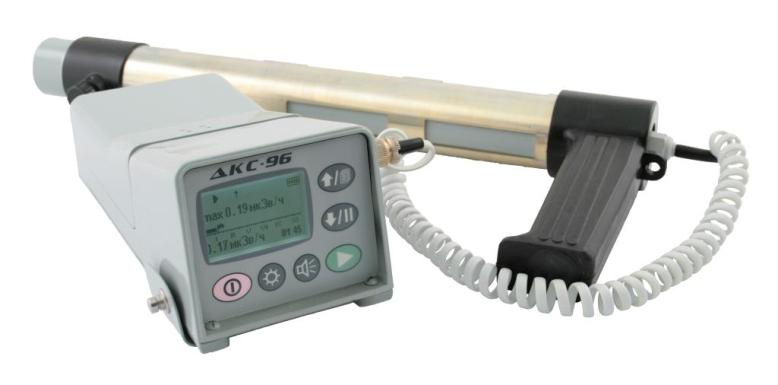
\includegraphics[width=0.4\textwidth]{DKS-96.jpg}
		\caption{Внешний вид ДКС-96}
	\end{figure}

    Дозиметр-радиометр в зависимости от типа подключенного блока детектирования 
    обеспечивает измерение:
    \begin{itemize}
    	\item[-] амбиентного эквивалента дозы (далее -- ЭД) непрерывного и 
    		импульсного рентгеновского и гамма -- излучений;
    	\item[-] мощности амбиентного эквивалента дозы (далее -- МЭД)
    		непрерывного и импульсного рентгеновского и гамма-излучений;
    	\item[-] амбиентного эквивалента дозы нейтронного излучения;
    	\item[-] мощности амбиентного эквивалента дозы нейтронного излучения;
    	\item[-] мощности экспозиционной дозы гамма-излучения;
    	\item[-] плотности потока альфа-излучения;
    	\item[-] плотности потока бета-излучения;
    	\item[-] плотности потока гамма-излучения;
    	\item[-] потока гамма-излучения;
    \end{itemize}

    Дозиметр-радиометр применяется в службах дозиметрического контроля на объектах 
    атомной энергетики и промышленности, в том числе на судах с ядерными энергетическими 
    установками, в медицинских, научных и других учреждениях, как самостоятельно, так 
    и в составе автоматизированных систем радиационного контроля:
    \begin{itemize}
    	\item[-] для оперативного и периодического контроля радиационной обстановки;
    	\item[-] для измерения уровня загрязненности поверхностей альфа-, бета- и 
    		гамма- активными веществами;
    	\item[-] для поиска и локализации источников ионизирующего излучения;
    	\item[-] для измерения потока гамма-излучения и мощности экспозиционной дозы 
    		гамма-излучения в скважинах и жидких средах;
    	\item[-] для контроля радиационного загрязнения металлолома;
    	\item[-] для радиационно-экологических исследований на участках строительства;
    	\item[-] в службах таможенного контроля при досмотре автотранспортных 
    		средств и грузов;
    \end{itemize}

\subsection{Принцип работы} \label{subsect2_2_3}
	В программе работы дозиметра-радиометра реализованы три алгоритма непрерывного 
	измерения физических величин, характеризующих регистрируемое ионизирующее 
	излучение:
	\begin{itemize}
		\item[-] <<С заданным временем>>;
		\item[-] <<С заданной точностью>>;
		\item[-] <<Следящий>>;
	\end{itemize}

	Алгоритм <<С заданным временем>> обеспечивает получение результата измерения, 
	равного текущему среднему значению с заданной экспозицией. Диапазон 
	допустимых значений экспозиции от 3 до 9999 с включительно.

	Алгоритм <<С заданной точностью>> обеспечивает получение результата 
	измерения с заданным <<по умолчанию>> значением неопределенности, равным 
	6\%. Расчёт неопределенности производится по формуле

	\begin{equation}
		u = \frac{2}{\sqrt{N}}\cdot 100
	\end{equation}

	где N -- количество зарегистрированных на текущий момент импульсов.

	Алгоритм <<Следящий>> -- обеспечивает получение результата измерения, 
	равного среднему арифметическому значению, рассчитанному методом 
	скользящего среднего по результатам N наблюдений с экспозицией, 
	равной одной секунде. 

\clearpage

\section{Радиометр радона РРА-01М-01} \label{sect2_4}
\subsection{Назначение} \label{subsect2_4_1}
    Радиометр РРА-01М-01 предназначен для экспрессных измерений объёмной 
    активности (далее -- ОА) радона-222 \( ^{222}Rn \) в воздухе жилых 
    и рабочих помещений, а также на открытом воздухе.

    \begin{figure}[ht]
		\centering
		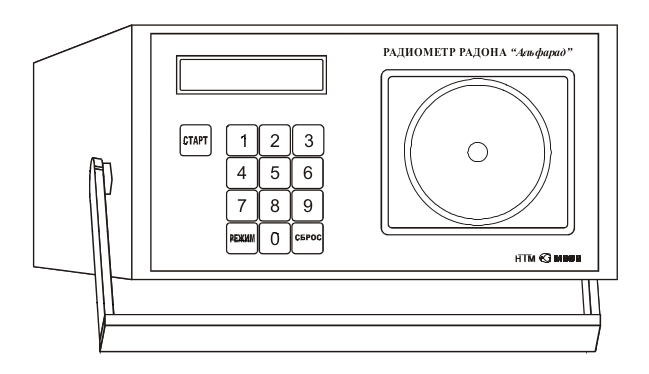
\includegraphics[width=0.5\textwidth]{RRA-01M-01.png}
		\caption{Внешний вид РРА-01М-01}
	\end{figure}

\subsection{Принцип работы} \label{subsect2_4_3}
    Измерение ОА радона-222 основано на электростатическом осаждении 
    заряженных ионов \( ^{218}Po \) (RaA) из отобранной пробы воздуха на 
    поверхности ППД. ОА \( ^{222}Rn \) определяется по количеству 
    зарегистрированных альфа-частиц при распаде атомов RaA, осевших на 
    ППД.

    Электрические импульсы, образующиеся под воздействием на детектор 
    альфа-частиц, усиливаются зарядочувствительным предусилителем и 
    поступают на вход амплитудно-цифрового преобразователя (далее АЦП) и 
    далее обрабатываются микропроцессором. Импульсы, соответствующие 
    альфа-частицам RaA, регистрируются счётчиком микропроцессора. Эффект, 
    обусловленных накоплением RaA на поверхности детектора, не влияет на 
    результаты последующих измерений в силу малого периода полураспада 
    RaA. Результаты измерений выводятся на матричный жидкокристаллический 
    дисплей.

\clearpage

\section{Установка спектрометрическая СКС-99 <<СПУТНИК>>} \label{section2_5}
\subsection{Назначение} \label{2_5_1}
    Установка спектрометрическая СКС-99 <<СПУТНИК>> МГФК.412154.001 
    (далее -- СКС-99), предназначена для спектрометрических, 
    радиометрических и дозиметрических измерений ионизирующих излучений. 

    СКС-99 может использоваться для решения широкого спектра задач 
    радиационного контроля от измерений в области сертификации соответствия 
    пищевой продукции, питьевой воды, строительных материалов, продукции 
    лесного хозяйства и др. до мониторинга и задач радиационного контроля 
    на предприятиях ядерного цикла, а также для решения целого ряда 
    исследовательских задач, связанных с измерениями радиоактивности.

    \begin{figure}[ht]
		\centering
		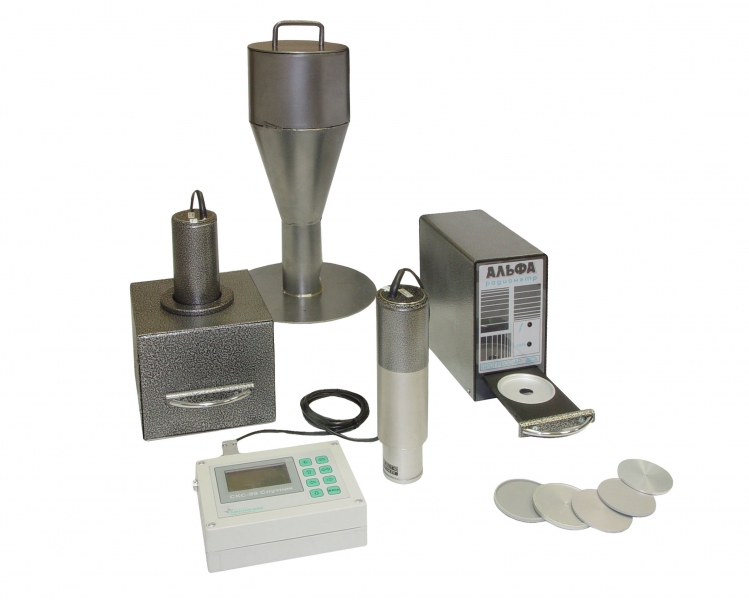
\includegraphics[width=0.4\textwidth]{CKC-99.jpg}
		\caption{Внешний вид СКС-99 <<СПУТНИК>>}
	\end{figure}

\subsection{Принцип работы} \label{2_4_3}
    Принцип работы СКС-99 основан на преобразовании энергии кванта 
    ионизирующего излучения в электрический импульс. Для гамма- и бета- 
    излучения амплитуды импульса пропорциональна энергии, потерянной 
    квантом в чувствительном объёме блока детектирования. Сигнал, 
    поступивший с блока детектирования, поступает на вход линейного 
    усилителя. Десятиразрядный АЦП преобразует сформированный усилителем 
    импульс и увеличивает количество отсчётов в соответствующем цифровому 
    коду канале на единицу.

    При работе в счётном режиме (альфа-радиометр и бета-счётчик) процессор 
    ведёт подсчёт количества пришедших импульсов независимо от их 
    амплитуды.

\clearpage